\documentclass{article}
\usepackage[english]{babel}
\usepackage[utf8]{inputenc}
\usepackage[english]{babel}
\usepackage[a4paper, total={7.25in, 9.5in}]{geometry}
\usepackage{tikz-feynman}
\tikzfeynmanset{compat=1.0.0} 
\usepackage{subcaption}
\usepackage{float}
\floatplacement{figure}{H}
\usepackage{simpler-wick}
\usepackage{mathrsfs}  
\usepackage{dsfont}
\usepackage{relsize}
\usepackage{tikz-cd}
\DeclareMathAlphabet{\mathdutchcal}{U}{dutchcal}{m}{n}

\usepackage{cancel}



\newcommand{\field}{\hat{\Phi}}
\newcommand{\dfield}{\hat{\Phi}^\dagger}
 
\usepackage{amsthm, amssymb, amsmath, centernot}
\usepackage{slashed}
\newcommand{\notimplies}{%
  \mathrel{{\ooalign{\hidewidth$\not\phantom{=}$\hidewidth\cr$\implies$}}}}
 
\renewcommand\qedsymbol{$\square$}
\newcommand{\cont}{$\boxtimes$}
\newcommand{\divides}{\mid}
\newcommand{\ndivides}{\centernot \mid}

\newcommand{\Integers}{\mathbb{Z}}
\newcommand{\Natural}{\mathbb{N}}
\newcommand{\Complex}{\mathbb{C}}
\newcommand{\Zplus}{\mathbb{Z}^{+}}
\newcommand{\Primes}{\mathbb{P}}
\newcommand{\Q}{\mathbb{Q}}
\newcommand{\R}{\mathbb{R}}
\newcommand{\ball}[2]{B_{#1} \! \left(#2 \right)}
\newcommand{\Rplus}{\mathbb{R}^+}
\renewcommand{\Re}[1]{\mathrm{Re}\left[ #1 \right]}
\renewcommand{\Im}[1]{\mathrm{Im}\left[ #1 \right]}
\newcommand{\Op}{\mathcal{O}}

\newcommand{\invI}[2]{#1^{-1} \left( #2 \right)}
\newcommand{\End}[1]{\text{End}\left( A \right)}
\newcommand{\legsym}[2]{\left(\frac{#1}{#2} \right)}
\renewcommand{\mod}[3]{\: #1 \equiv #2 \: \mathrm{mod} \: #3 \:}
\newcommand{\nmod}[3]{\: #1 \centernot \equiv #2 \: mod \: #3 \:}
\newcommand{\ndiv}{\hspace{-4pt}\not \divides \hspace{2pt}}
\newcommand{\finfield}[1]{\mathbb{F}_{#1}}
\newcommand{\finunits}[1]{\mathbb{F}_{#1}^{\times}}
\newcommand{\ord}[1]{\mathrm{ord}\! \left(#1 \right)}
\newcommand{\quadfield}[1]{\Q \small(\sqrt{#1} \small)}
\newcommand{\vspan}[1]{\mathrm{span}\! \left\{#1 \right\}}
\newcommand{\galgroup}[1]{Gal \small(#1 \small)}
\newcommand{\bra}[1]{\left| #1 \right>}
\newcommand{\Oa}{O_\alpha}
\newcommand{\Od}{O_\alpha^{\dagger}}
\newcommand{\Oap}{O_{\alpha '}}
\newcommand{\Odp}{O_{\alpha '}^{\dagger}}
\newcommand{\im}[1]{\mathrm{im} \: #1}
\renewcommand{\ker}[1]{\mathrm{ker} \: #1}
\newcommand{\ket}[1]{\left| #1 \right>}
\renewcommand{\bra}[1]{\left< #1 \right|}
\newcommand{\inner}[2]{\left< #1 | #2 \right>}
\newcommand{\expect}[2]{\left< #1 \right| #2 \left| #1 \right>}
\renewcommand{\d}[1]{ \mathrm{d}#1 \:}
\newcommand{\dn}[2]{ \mathrm{d}^{#1} #2 \:}
\newcommand{\deriv}[2]{\frac{\d{#1}}{\d{#2}}}
\newcommand{\nderiv}[3]{\frac{\dn{#1}{#2}}{\d{#3^{#1}}}}
\newcommand{\pderiv}[2]{\frac{\partial{#1}}{\partial{#2}}}
\newcommand{\fderiv}[2]{\frac{\delta #1}{\delta #2}}
\newcommand{\parsq}[2]{\frac{\partial^2{#1}}{\partial{#2}^2}}
\newcommand{\topo}{\mathcal{T}}
\newcommand{\base}{\mathcal{B}}
\renewcommand{\bf}[1]{\mathbf{#1}}
\renewcommand{\a}{\hat{a}}
\newcommand{\adag}{\hat{a}^\dagger}
\renewcommand{\b}{\hat{b}}
\newcommand{\bdag}{\hat{b}^\dagger}
\renewcommand{\c}{\hat{c}}
\newcommand{\cdag}{\hat{c}^\dagger}
\newcommand{\hamilt}{\hat{H}}
\renewcommand{\L}{\hat{L}}
\newcommand{\Lz}{\hat{L}_z}
\newcommand{\Lsquared}{\hat{L}^2}
\renewcommand{\S}{\hat{S}}
\renewcommand{\empty}{\varnothing}
\newcommand{\J}{\hat{J}}
\newcommand{\lagrange}{\mathcal{L}}
\newcommand{\dfourx}{\mathrm{d}^4x}
\newcommand{\meson}{\phi}
\newcommand{\dpsi}{\psi^\dagger}
\newcommand{\ipic}{\mathrm{int}}
\newcommand{\tr}[1]{\mathrm{tr} \left( #1 \right)}
\newcommand{\C}{\mathbb{C}}
\newcommand{\CP}[1]{\mathbb{CP}^{#1}}
\newcommand{\Vol}[1]{\mathrm{Vol}\left(#1\right)}

\newcommand{\Tr}[1]{\mathrm{Tr}\left( #1 \right)}
\newcommand{\Charge}{\hat{\mathbf{C}}}
\newcommand{\Parity}{\hat{\mathbf{P}}}
\newcommand{\Time}{\hat{\mathbf{T}}}
\newcommand{\Torder}[1]{\mathbf{T}\left[ #1 \right]}
\newcommand{\Norder}[1]{\mathbf{N}\left[ #1 \right]}
\newcommand{\Znorm}{\mathcal{Z}}
\newcommand{\EV}[1]{\left< #1 \right>}
\newcommand{\interact}{\mathrm{int}}
\newcommand{\covD}{\mathcal{D}}
\newcommand{\conj}[1]{\overline{#1}}

\newcommand{\SO}[2]{\mathrm{SO}(#1, #2)}
\newcommand{\SU}[2]{\mathrm{SU}(#1, #2)}

\newcommand{\anticom}[2]{\left\{ #1 , #2 \right\}}


\newcommand{\pathd}[1]{\! \mathdutchcal{D} #1 \:}

\renewcommand{\theenumi}{(\alph{enumi})}


\renewcommand{\theenumi}{(\alph{enumi})}

\newcommand{\atitle}[1]{\title{% 
	\large \textbf{Physics GR8048 Quantum Field Theory II
	\\ Assignment \# #1} \vspace{-2ex}}
\author{Benjamin Church }
\maketitle}

\newcommand{\atitleIII}[1]{\title{% 
	\large \textbf{Physics GR8049 Quantum Field Theory III
	\\ Assignment \# #1} \vspace{-2ex}}
\author{Benjamin Church }
\maketitle}

\theoremstyle{definition}
\newtheorem{theorem}{Theorem}[section]
\newtheorem{definition}{definition}[section]
\newtheorem{lemma}[theorem]{Lemma}
\newtheorem{proposition}[theorem]{Proposition}
\newtheorem{corollary}[theorem]{Corollary}
\newtheorem{example}[theorem]{Example}
\newtheorem{remark}[theorem]{Remark}

\usepackage{relsize}
\begin{document}

\begin{equation*}
\begin{tikzpicture}[baseline = -0.11cm]
\begin{feynman}
\vertex (a);
\vertex [above left=of a, momentum = $p_1$] (i1) ;
\vertex [below left=of a, rmomentum = $p_2$] (i2) 
;
\vertex [right=of a, blob] (b) {\(\mathbf{1PI}\)};
\vertex [right=of b] (c);
\vertex [above right=of c] (f1) ;
\vertex [below right=of c] (f2) ;
\diagram* {
(i1) --[fermion, momentum = $p_1$] (a) -- [fermion, rmomentum = $p_2$] (i2),
(a) -- [scalar] (b) -- [scalar] (c)
(f2) --[fermion, rmomentum = $p_1'$] (c) -- [fermion, momentum = $p_2'$] (f1)
};
\end{feynman}
\end{tikzpicture}
\quad 
+
\quad 
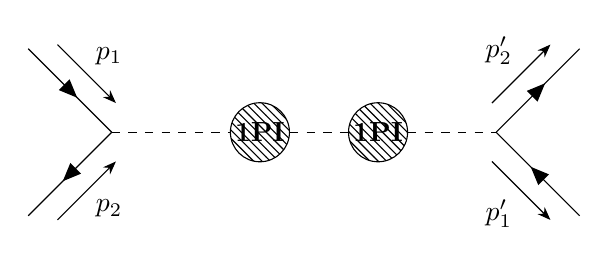
\begin{tikzpicture}[baseline = -0.11cm]
\begin{feynman}
\vertex (a);
\vertex [above left=of a, momentum = $p_1$] (i1) ;
\vertex [below left=of a, rmomentum = $p_2$] (i2) ;
\vertex [right=of a, blob] (b) {\(\mathbf{1PI}\)};
\vertex [right=of b, blob] (c) {\(\mathbf{1PI}\)};
\vertex [right=of c] (d);
\vertex [above right=of d] (f1) ;
\vertex [below right=of d] (f2) ;
\diagram* {
(i1) --[fermion, momentum = $p_1$] (a) -- [fermion, rmomentum = $p_2$] (i2),
(a) -- [scalar] (b) -- [scalar] (c) -- [scalar] (d),
(f2) --[fermion, rmomentum = $p_1'$] (d) -- [fermion, momentum = $p_2'$] (f1)
};
\end{feynman}
\end{tikzpicture}
\end{equation*}
\begin{equation*}
\quad 
+
\quad 
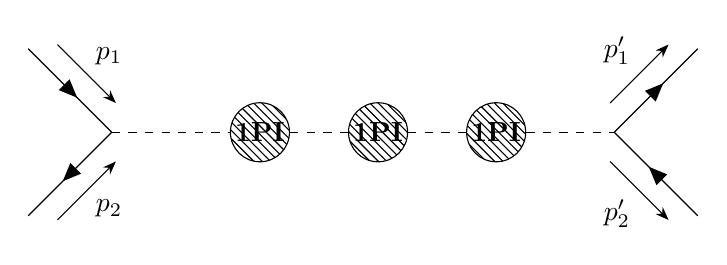
\begin{tikzpicture}[baseline = -0.11cm]
\begin{feynman}
\vertex (a);
\vertex [above left=of a] (i1) ;
\vertex [below left=of a] (i2) ;
\vertex [right=of a, blob] (b) {\(\mathbf{1PI}\)};
\vertex [right=of b, blob] (c) {\(\mathbf{1PI}\)};
\vertex [right=of c, blob] (d) {\(\mathbf{1PI}\)};
\vertex [right=of d] (e);
\vertex [above right=of e] (f1) ;
\vertex [below right=of e] (f2) ;
\diagram* {
(i1) --[fermion, momentum = $p_1$] (a) -- [fermion, rmomentum = $p_2$] (i2),
(a) -- [scalar] (b) -- [scalar] (c) -- [scalar] (d) -- [scalar] (e),
(f2) --[fermion, rmomentum = $p_2'$] (e) -- [fermion, momentum = $p_1'$] (f1)
};
\end{feynman}
\end{tikzpicture}
\quad
+ 
\quad
\cdots
\end{equation*}
and similarly,
\begin{equation*}
\begin{tikzpicture}[baseline = -2cm]
\begin{feynman}
\vertex (a);
\vertex [above left=of a, momentum' = $p_1$] (i1) ;
\vertex [above right=of a, rmomentum = $p_2$] (i2) 
;
\vertex [below=of a, blob] (b) {\(\mathbf{1PI}\)};
\vertex [below=of b] (c);
\vertex [below left=of c] (f1) ;
\vertex [below right=of c] (f2) ;
\diagram* {
(i1) --[fermion, momentum' = $p_1$] (a) -- [fermion, momentum' = $p_1'$] (i2),
(a) -- [scalar] (b) -- [scalar] (c)
(f2) --[fermion, rmomentum' = $p_2'$] (c) -- [fermion, rmomentum' = $p_2$] (f1)
};
\end{feynman}
\end{tikzpicture}
\quad 
+
\quad 
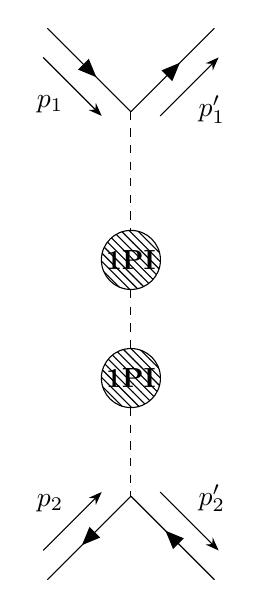
\begin{tikzpicture}[baseline = -2.5cm]
\begin{feynman}
\vertex (a);
\vertex [above left=of a, momentum' = $p_1$] (i1) ;
\vertex [above right=of a, rmomentum = $p_2$] (i2) 
;
\vertex [below=of a, blob] (b) {\(\mathbf{1PI}\)};
\vertex [below=of b, blob] (c) {\(\mathbf{1PI}\)};
\vertex [below=of c] (d);
\vertex [below left=of d] (f1) ;
\vertex [below right=of d] (f2) ;
\diagram* {
(i1) --[fermion, momentum' = $p_1$] (a) -- [fermion, momentum' = $p_1'$] (i2),
(a) -- [scalar] (b) -- [scalar] (c) -- [scalar] (d),
(f2) --[fermion, rmomentum' = $p_2'$] (d) -- [fermion, rmomentum' = $p_2$] (f1)
};
\end{feynman}
\end{tikzpicture}
\quad 
+
\quad 
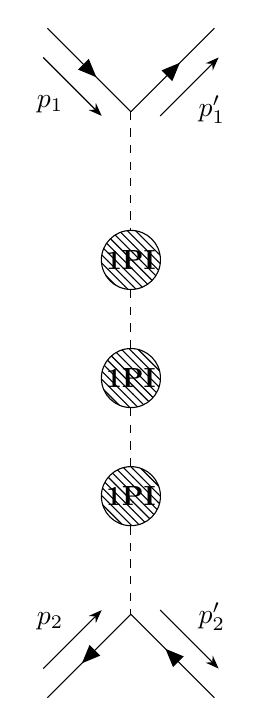
\begin{tikzpicture}[baseline = -3cm]
\begin{feynman}
\vertex (a);
\vertex [above left=of a, momentum' = $p_1$] (i1) ;
\vertex [above right=of a, rmomentum = $p_2$] (i2) 
;
\vertex [below=of a, blob] (b) {\(\mathbf{1PI}\)};
\vertex [below=of b, blob] (c) {\(\mathbf{1PI}\)};
\vertex [below=of c, blob] (d) {\(\mathbf{1PI}\)};
\vertex [below=of d] (e);
\vertex [below left=of e] (f1) ;
\vertex [below right=of e] (f2) ;
\diagram* {
(i1) --[fermion, momentum' = $p_1$] (a) -- [fermion, momentum' = $p_1'$] (i2),
(a) -- [scalar] (b) -- [scalar] (c) -- [scalar] (d) -- [scalar] (e),
(f2) --[fermion, rmomentum' = $p_2'$] (e) -- [fermion, rmomentum' = $p_2$] (f1)
};
\end{feynman}
\end{tikzpicture}
\quad
+ 
\quad
\cdots
\end{equation*}
\end{document}
